\documentclass[journal,12pt,twocolumn]{IEEEtran}
\usepackage{graphicx}
\usepackage[margin=0.5in]{geometry}
\usepackage[cmex10]{amsmath}
\usepackage{array}
\usepackage{booktabs}
\usepackage{mathtools}
\usepackage{hyperref}


\title{\textbf{Optimization Assignment - 1}}
\author{Mandava.Gowthami}
\date{October 2022}


\providecommand{\norm}[1]{\left\lVert#1\right\rVert}
\providecommand{\abs}[1]{\left\vert#1\right\vert}
\let\vec\mathbf
\newcommand{\myvec}[1]{\ensuremath{\begin{pmatrix}#1\end{pmatrix}}}
\newcommand{\mydet}[1]{\ensuremath{\begin{vmatrix}#1\end{vmatrix}}}
\providecommand{\brak}[1]{\ensuremath{\left(#1\right)}}
\providecommand{\lbrak}[1]{\ensuremath{\left(#1\right.}}
\providecommand{\rbrak}[1]{\ensuremath{\left.#1\right)}}
\providecommand{\sbrak}[1]{\ensuremath{{}\left[#1\right]}}

\begin{document}
\maketitle

\section{Question}
For
\textbf{x} \in \sbark({0,5\pi/2})\;define\;
$f(x)=\int_{0}^{x} \sqrt{t}sint\,dt$}\;
.Then \textbf{f} has
 \section{Solution}
 \textbf{STEP-1}
 The given function \textbf{f(x)} is defined in given range and derivative of this fuction exists.\\
  \textbf{STEP-2}
 we can find the maxima of \textbf{f(x)} by using gradient ascent method
 
$\implies x_{n+1} = x_n + \alpha \nabla f(x_n) $\\
 \begin{align}
        \implies x_{n+1} &= x_n + \alpha \brak{\sqrt{x}sinx}
    \end{align}
 Taking $x_0=0.5,\alpha=0.001$ and precision = 0.00000001, values obtained using python are:
    
    \begin{align}
        \boxed{\text{Maxima} = 9.9979e-06}\\
        \boxed{\text{Maxima Point} = 3.141}
    \end{align}
 
 \textbf{STEP-3}
 we can find the minima of eq(1) by using gradient descent method
 
$\implies x_{n+1} = x_n - \alpha \nabla f(x_n) $\\
 \begin{align}
        \implies x_{n+1} &= x_n - \alpha \brak{\sqrt{x}sinx}
    \end{align}
Taking $x_0=4,\alpha=0.001$ and precision = 0.00000001, values obtained using python are:
    
    \begin{align}
        \boxed{\text{Minima} =-09.9951e-06}\\
        \boxed{\text{Minima Point} = 6.283}
    \end{align}
\begin{figure}[h!]
\centering
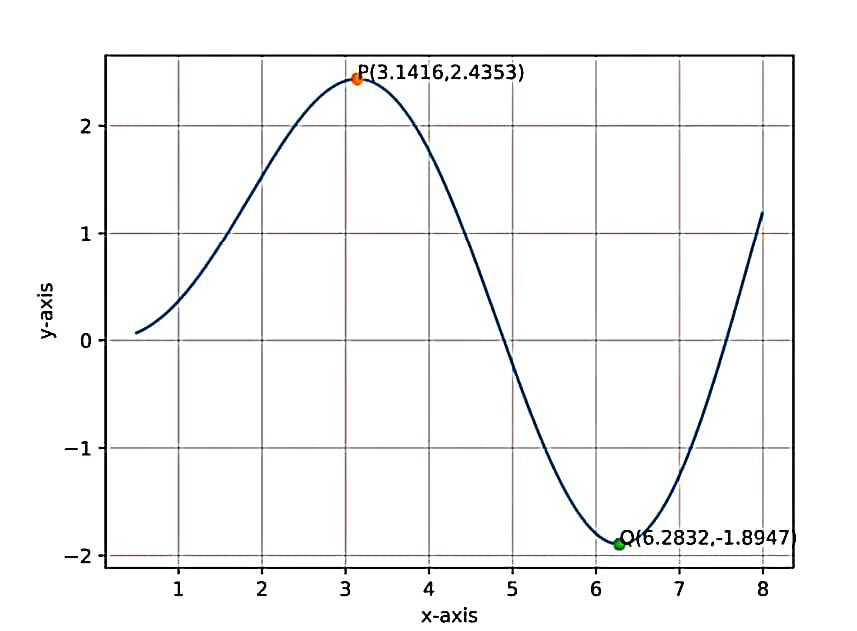
\includegraphics[scale=0.3]{pic.jpg}  \\
\caption{plot of f(x) with maxima and minima points}
\end{figure}
    
Get the python code of the figures from
\begin{table}[h]
\large
\centering
\framebox{
\url{https://github.com/gowthami/GOWTHAMI_FWC/blob/main/optimization_1/code/optimization1.py}}
\bibliographystyle{ieeetr}
\end{table}
 
\end{document}
